\documentclass[]{tukediphc}
%% -----------------------------------------------------------------
%% tento subor ma kodovanie utf-8
%%
%% na kompilaciu pouzivajte format pdfcslatex 
%%
%% vytvorene distribuciou texlive 2009-7, OS GNU/Linux
%% vytvorene distribuciou TeXLive 2010, OS Win XP
%% februar 2013
%% -----------------------------------------------------------------
\usepackage[utf8]{inputenc}
%\usepackage[T1]{fontenc}
\usepackage{lmodern,textcase}
\usepackage[slovak]{babel}\renewcommand{\figurename}{Obr\'azok}
\def\refname{Zoznam pou\v{z}itej literat\'ury}
\usepackage{latexsym}
\usepackage{dcolumn} % zarovnanie cisiel v tabulke podla des. ciarky
\usepackage{hhline}
\usepackage{subfig}
\usepackage{amsmath}
\usepackage{nicefrac} % pekne zlomky
\usepackage{upgreek} % napr. $\upmu\mathrm{m}$ pre mikrometer ...
\usepackage[final]{showkeys}%color%notref%notcite%final
\usepackage[slovak,noprefix]{nomencl}
\makeglossary % prikaz na vytvorenie suboru .glo
\usepackage{parskip}% 'zhusti' polozky obsahu
%%
%\usepackage[dvips]{graphicx}
%\DeclareGraphicsExtensions{.eps}
\usepackage[pdftex]{graphicx}
\DeclareGraphicsExtensions{.pdf,.png,.jpg,.mps}
\graphicspath{{figures/}} % priecinok na obrazky
%%
%% Cislovane citovanie
%\usepackage[numbers]{natbib}
%%
%% Citovanie podľa mena autora a roku
\usepackage{natbib} \citestyle{chicago}
% -----------------------------------------------------------------
%% tlač !!!
\usepackage[pdftex,unicode=true,bookmarksnumbered=true,
bookmarksopen=true,pdfmenubar=true,pdfview=Fit,linktocpage=true,
pageanchor=true,bookmarkstype=toc,pdfpagemode=UseOutlines,
pdfstartpage=1]{hyperref}
\hypersetup{%
baseurl={http://www.tuke.sk/sevcovic},
pdfcreator={pdfcsLaTeX},
pdfkeywords={Riadenie procesov, Oceliarstvo, Vizualizácia, Virtuálna realita, Matematické modelovanie},
pdftitle={Písomná príprava k predmetu Matematické metódy identifikácie, modelovania a simulácie},
pdfauthor={Michal Takáč},
pdfsubject={Dizertačná skúška}
} 
%% nehodiace zakomentujte !
%\dippraca{Písomná príprava k predmetu Riadenie procesov}
%\bakpraca{Príprava na dizertačnú skúšku}
%%
\nazov{Písomná príprava k predmetu Matematické metódy identifikácie, modelovania a simulácie}
%% ked praca nema 'podnazov' zakomentujte nasledujuci riadok
%% alebo polozku nechajte prazdnu
\podnazov{}
\autor{Ing.~Michal Takáč}
\veduciprace{prof.~RNDr.~Igor~Podlubný, DrSc.}
\univerzita{Technická univerzita v~Košiciach}
\fakulta{Fakulta baníctva, ekológie, riadenia a geotechnológií}
\skratkafakulty{FBERG}
\katedra{Ústav riadenia a informatizácie výrobných procesov}
\skratkakatedry{URIVP}
\odbor{Riadenie procesov}
\specializacia{Kybernetika}
\abstrakt{Abstrakt je povinnou súčasťou každej práce. Je výstižnou
charakteristikou obsahu dokumentu. Nevyjadruje hodnotiace stanovisko
autora. Má byť\/ taký informatívny, ako to povoľuje podstata práce.
Text abstraktu sa píše ako jeden odstavec. Abstrakt neobsahuje odkazy
na samotný text práce. Mal by mať\/ rozsah 250 až 500 slov. Pri
štylizácii sa používajú celé vety, slovesá v činnom rode a tretej
osobe. Používa sa odborná terminológia, menej zvyčajné termíny,
skratky a~symboly sa pri prvom výskyte v texte definujú.}
\klucoveslova{Riadenie procesov, Oceliarstvo, Vizualizácia, Virtuálna realita, Matematické modelovanie}
\datumodovzdania{30. 5. 2020}
\mesto{Košice}

\begin{document}
\renewcommand\theHfigure{\theHsection.\arabic{figure}}
\renewcommand\theHtable{\theHsection.\arabic{table}}
\bibliographystyle{dcu}

\prvastrana


\thispagestyle{empty}
\tableofcontents
\newpage
%
%\thispagestyle{empty}
%%\addcontentsline{toc}{section}{\numberline{}Zoznam obrázkov}
%\listoffigures
%\newpage
%
%\thispagestyle{empty}
%%\addcontentsline{toc}{section}{\numberline{}Zoznam tabuliek}
%\listoftables
%\newpage

%%%%%%%%%%%%%%%%%%%%%%%%%%%%%%%%%

\setcounter{page}{1}
\setcounter{equation}{0}
\setcounter{figure}{0}
\setcounter{table}{0}

\section{Úvod}

V kyslíkovom konvertore prebieha množstvo chemických reakcií a fyzikálnych javov, medzi ktorými sa nájdu aj také, ktorým úplne nerozumieme z dôvodu ich komplexnosti. Podstatou výroby ocele v takomto konvertore je oxidácia prvkov z kovonosnej vsádzky s kyslíkom fúkaným do konvertora. Oxidy týchto prvkov prechádzajú do trosky alebo odchádzajú vo forme konvertorového plynu. V kombinácii s fúkaním kyslíka prebieha proces miešania, aby sa podporila defosforizácia, dekarbonizácia, zahrievanie roztavenej ocele a homogenizácia zloženia a teploty ocele.

Rýchla dynamika procesu výroby ocele kyslíkovým konvertorom sťažuje dosiahnutie stabilných podmienok pre fúkanie kyslíka a súčasne dosiahnutie požadovaného zloženia ocele a teploty v koncovom bode tavenia. Nelineárna povaha chemických a termodynamických procesov pri výrobe ocele v LD konvertore tiež vzbudila záujem o vývoj nových matematických modelov založených na neceločíselnom diferenciálnom počte.

Matematický model predstavuje súbor funkčných vzťahov, ktoré transformujú vstupné hodnoty na výsledky, ktorými je možné vyjadriť podstatu modelovaného deja. Modelovanie je pravdepodobne najdôležitejšia časť procesu simulácie. Jej cieľom je čo najpresnejšie zachytiť správanie sa reálneho systému. Zahŕňa identifikáciu problému a očakávaný cieľ riešenia problému, zber reálnych dát alebo generácia náhodných dát, vytvorenie modelu, jeho úprava, prispôsobovanie a jeho overenie porovnaním výstupných dát zo simulácie s reálnymi dátami z reálneho systému.

\section{Počítačom podporované matematické modelovanie}

Počítačom podporované inžinierstvo (CAE - Computer Aided Engineering) je použitie počítačového softvéru na simuláciu výkonu s cieľom vylepšiť návrhy výrobkov alebo pomôcť pri riešení technických problémov pre celý rad priemyselných odvetví. To zahŕňa simuláciu, validáciu a optimalizáciu produktov, procesov a výrobných nástrojov.

Typický proces CAE pozostáva z krokov predbežného spracovania, riešenia a následného spracovania. Vo fáze predspracovania inžinieri modelujú geometriu (alebo reprezentáciu systému) a fyzikálne vlastnosti návrhu, ako aj prostredie vo forme aplikovaného zaťaženia alebo obmedzení. Ďalej je model vyriešený pomocou vhodnej matematickej formulácie základnej fyziky. Vo fáze po spracovaní sa výsledky predložia technikovi na preskúmanie.

V metalurgii pri výrobe ocele je veľmi dôležité simulovať lineárne a nelineárne procesy, s ktorými sa pri výrobe ocele stretávame pri tvorbe matematických modelov. Motivácia na používanie počítačových simulácií na skúmanie metalurgických procesov je dvojaká. Po prvé, umožňuje testovať zmeny dizajnu pred vytvorením prototypu, čo samozrejme vedie k nižším celkovým nákladom na návrh. Po druhé, umožňuje skúmať javy, ktoré sa nedajú ľahko merať alebo pozorovať v procese. Dokonca aj zdanlivo jednoduchá operácia, ako napríklad nepretržité meranie teploty počas procesu oduhličovania, je zložitá z dôvodu veľmi vysokých teplôt v procese a všeobecne drsných podmienok prevládajúcich v oceliarňach \citep{Ersson2018}.

Problémy s modernou mechanikou tekutín by nebolo možné vyriešiť bez použitia počítačovej dynamiky tekutín (CFD - Computational Fluid Dynamics). CFD je vetva CAE, ktorá sa zaoberá simuláciou pohybu tekutín a prenosom tepla pomocou numerických prístupov, pretože rozsah analytických riešení základných rovníc mechaniky tekutín je veľmi obmedzený a hlavne veľmi obtiažny. V prípade zložitejšej geometrie to znamená, že je výhodnejšie zvoliť numerickú metódu. 

\section{Počítačová dynamika tekutín (CFD)}

Počítačová dynamika tekutín (CFD) je využívaná od začiatku 20. storočia v oboroch fyziky akými sú aerodynamika, termodynamika alebo hydrodynamika. Je založená na numerickom riešení modelovanej sústavy parciálnych diferenciálnych rovníc, ktore popisujú určité formy pohybu a ktoré vyjadrujú zákon zachovania hmotnosti (rovnica kontinuity), zákon zachovania hybnosti (Navier-Stokesove rovnice) a zákon zachovania energie (rovnice prenosu tepla konvekciou, kondukciou alebo radiáciou).

Pri skúmaní dynamických javov tekutín je cieľom CFD analýzy vytvoriť čo najpresnejší obraz o týchto javoch a procesoch, ktoré vznikajú a prebiehajú pri pohybe plynných a kvapalných látok v okolí alebo vo vnútri objektov v pevnom skupenstve. Presnosť CFD simulácií ale nie je zaručená a tak treba stále počítať s tým, že nám vedia poskytnúť iba približné informácie o tom, ako sa bude simulovaná súčiastka alebo proces správať v reálnom svete. 

Pohyb tekutín súvisí s rôznymi problémami danými fyzikálnym modelom, ako napríklad laminárne a turbulentné prúdenie, stlačiteľné a nestlačiteľné prúdenie, prenos a distribúcia tepla, prenos chemických prímesí vrátane chemických reakcií, viacfázové prúdenie, prúdenie poréznym prostredím, vznik bublín alebo horenie.

Metódami numerickej matematiky, formuláciou okrajových a počiatočných podmienok sa z úlohy mechaniky tekutín formuluje matematický problém. Z formulácie určujúcich rovníc (fyzikálny model), ktoré sa spravidla nedajú riešiť analyticky, sa diskretizáciou získajú algebraické rovnice (matematický model). Okrajové podmienky určujú, ako systém (napríklad štruktúra alebo tekutina) interaguje s prostredím. Fixácie, zaťaženia, tlaky, prietok alebo rýchlosť tekutiny sú príklady okrajových podmienok. Počiatočné podmienky definujú počiatočné hodnoty pre každé pole riešenia a sú vyjadrené fyzikálnymi veličinami. V priebehu riešenia sa menia každou iteráciou. Majú vplyv na čas dosiahnutia konvergencie riešenia úlohy, tj. dobu výpočtu. Samotná úloha je taktiež určená geometrickou štruktúrou (geometrický model).

V prvých štádiách nastavenia simulácie je potrebné definovať a vymedziť skúmanú oblasť v 2D alebo 3D, ktorá zahŕňa predmet modelovania a jeho najbližšie okolie. Táto oblasť sa pokryje sieťou (softvér to vie spraviť automaticky), to znamená, že sa rozdelí do určitého počtu 2D alebo 3D buniek (elementov). Počet buniek môže byť na rôznych miestach variabilný - to, koľkými bunkami je tvorená časť priestoru udáva, ako presná bude simulácia v danej oblasti. Detailnosť siete určuje aj čas výpočtov (čím detailnejšia, tým je simulácia zdĺhavejšia). Fyzikálne veličiny sú počítané pre geometrický stred každej bunky, hodnoty v ostatných miestach buniek sú interpolované alebo extrapolované.

\subsection{CFD v metalurgii}

Od počiatku priekopníckej práce v oblasti metalurgie, ktorú uskutočnili Szekely a kol. (1977), bolo vyvinutých veľa modelov, konkrétne pre kyslíkové konvertory to boli modely procesu zmiešavania, napenenia trosky, interakcií plyn-kvapalina, viacfázových tokov, ako aj aspektov prenosu tepla a hmoty \citep{chattopadhyay2010}. Náklady na vykonávanie počítačových simulácií sa za posledných niekoľko desaťročí znížili, zatiaľ čo dostupný výpočtový výkon sa zvýšil. Súčasne dostupné procesory sú štandardne viacjadrové, vďaka čomu je možné vykonávať viacero výpočtov súbežne. Pre zložité výpočty sa začali využívať grafické výpočtové jednotky (GPU) kvôli možnej paralelizácii výpočtových algoritmov. Štúdia z posledných dvoch desaťročí \citep{Ersson2018} využívania CFD simulácií v metalurgii odhaľuje obrovské zlepšenie týkajúce sa typu javov, ktoré je možné vďaka  nim preskúmať a tento trend bude  aj naďalej pokračovať. Ich použitie v oceliarskom priemysle však ešte stále nie je tak intenzívne ako v leteckom a automobilovom priemysle, v ktorých je vývoj nových dizajnov kľúčový. Hlavný rozdiel medzi leteckým a metalurgickým priemyslom spočíva v tom, že metalurgia sa takmer vždy zaoberá viacfázovými systémami pri zvýšených teplotách a že motiváciou modelovania je najmä optimalizácia procesov. S pokračujúcim vývojom vo viacfázových modeloch, ako aj pri reakčnom modelovaní toku, je užitočnosť CFD v metalurgii jasná.

\begin{figure}[!ht]
	\centering
	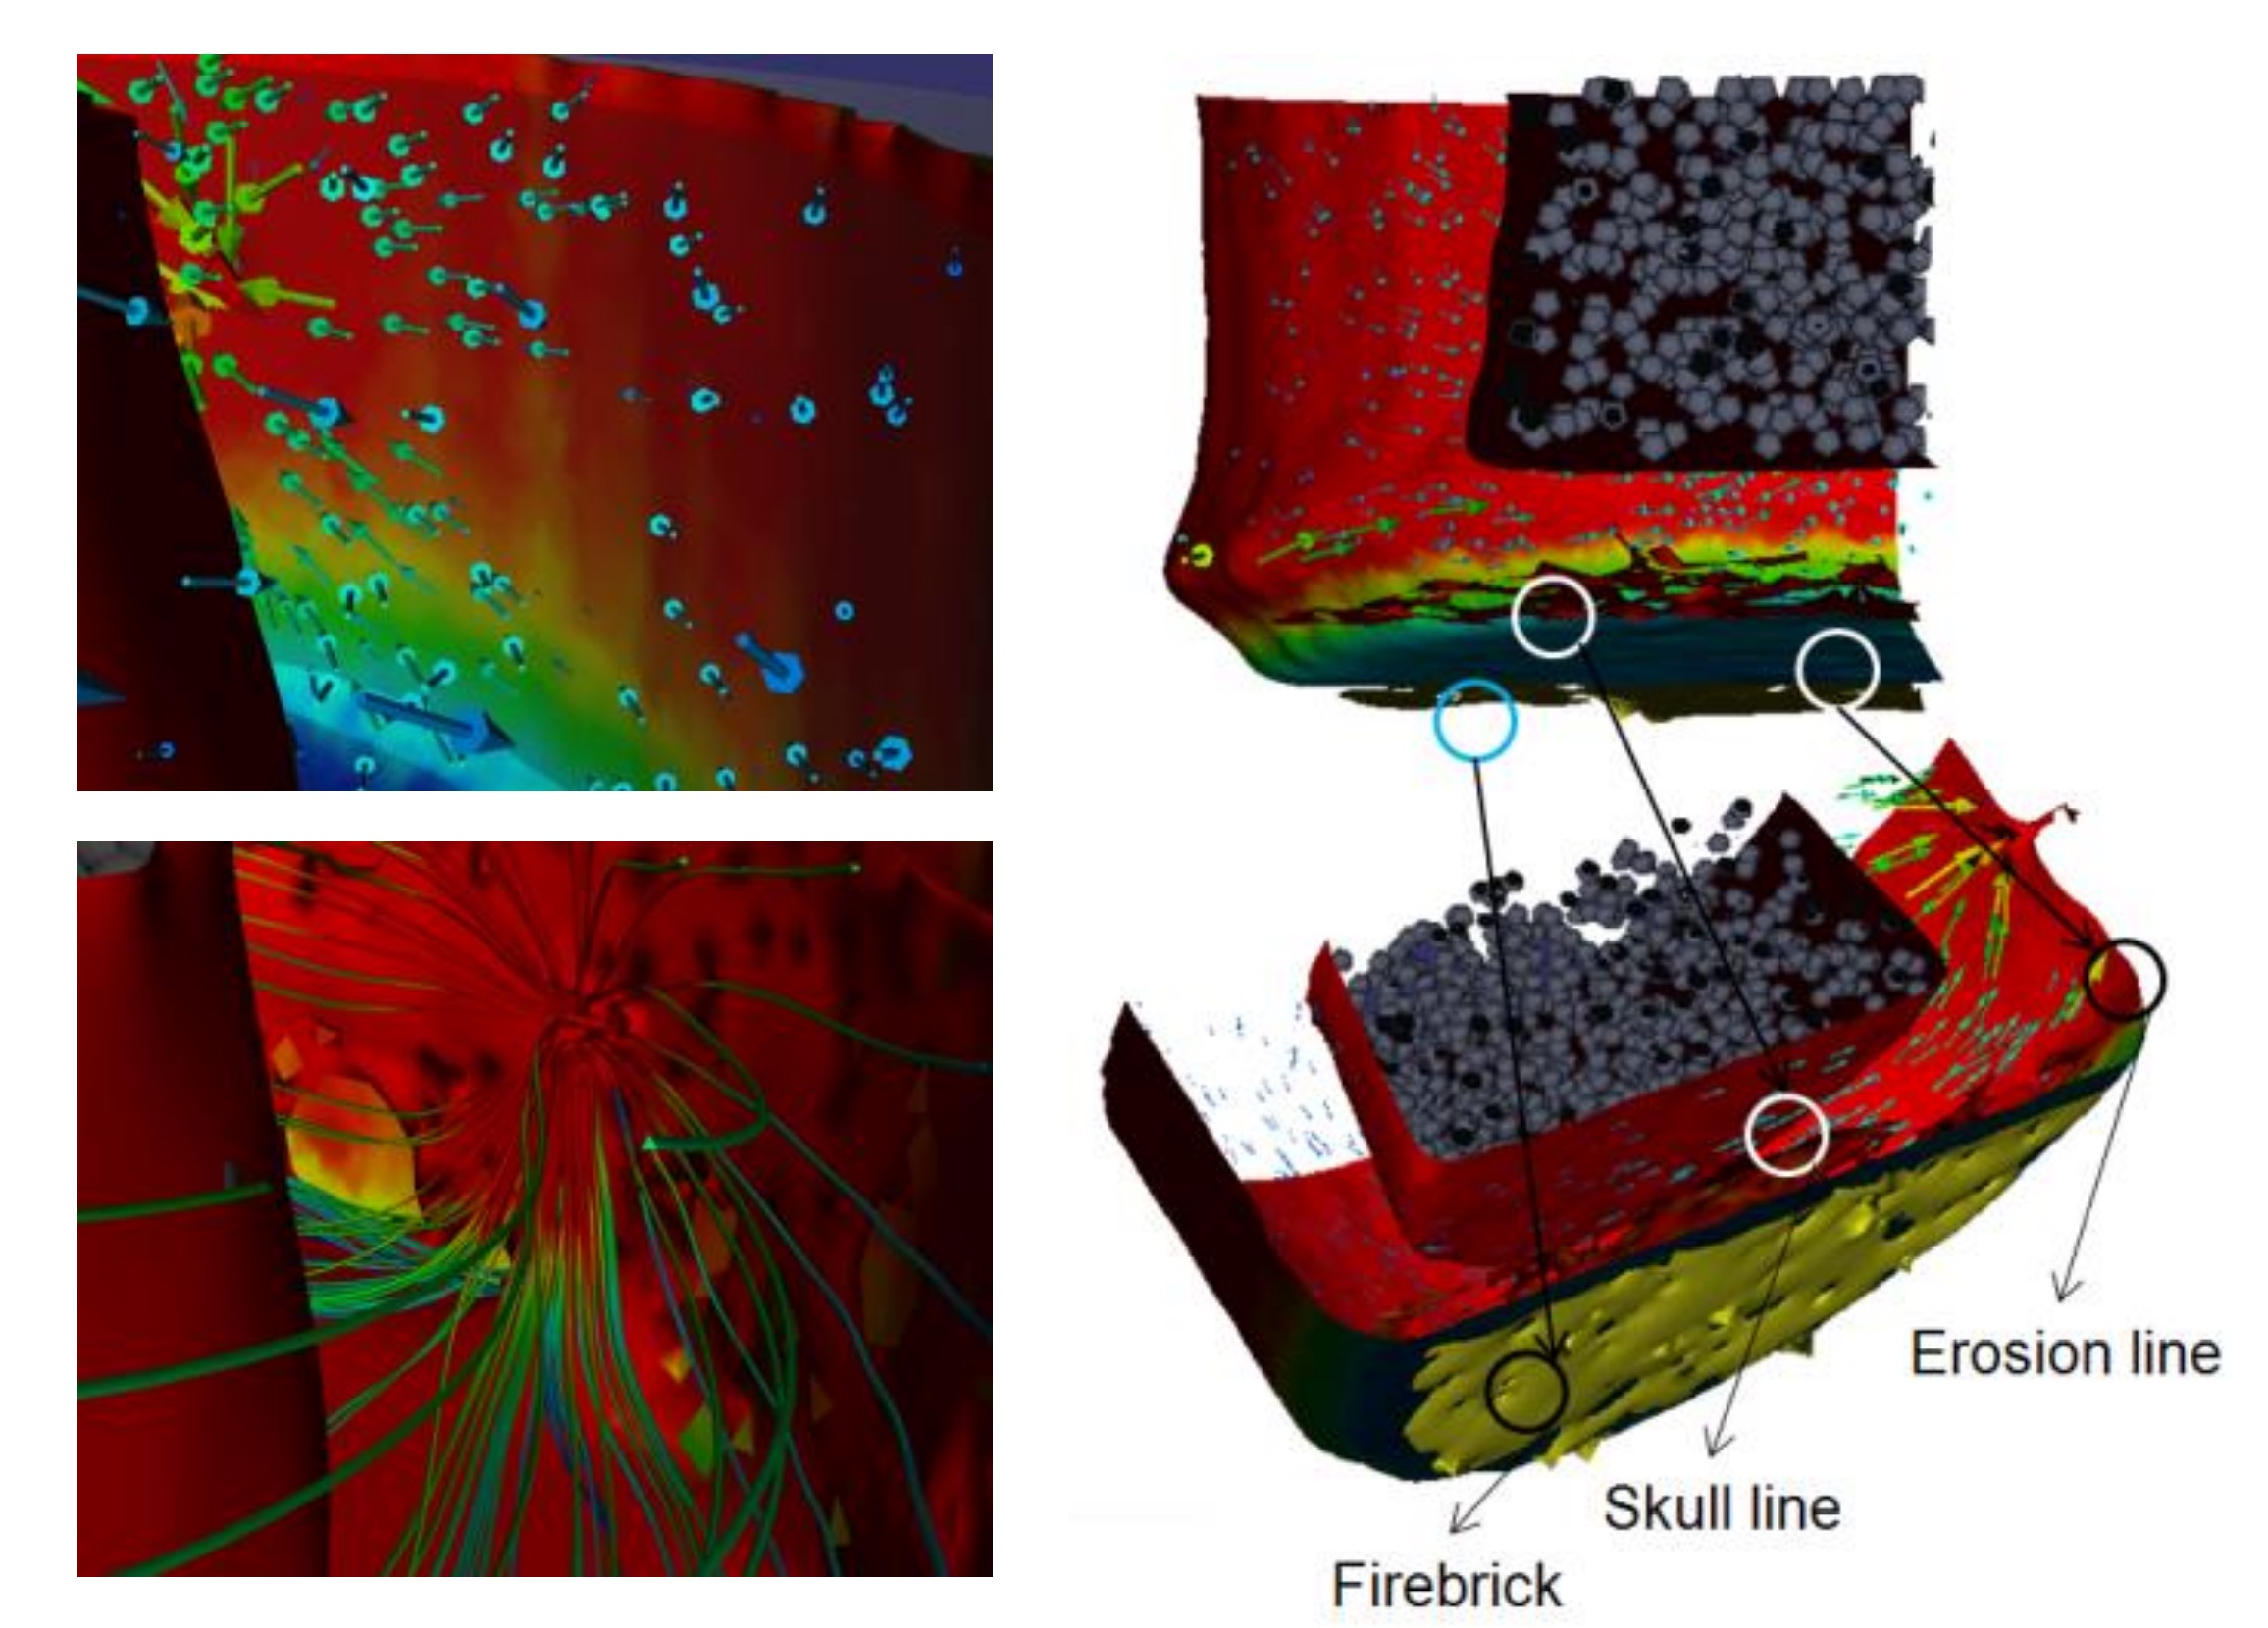
\includegraphics[width=.8\textwidth,angle=0]{figures/blast-furnace-erosion-vr.jpg}
	\caption{3D CFD simulácia a vizualizácia vnútra ("srdca") vysokej pece.}
\end{figure}

Pri numerických simuláciách procesov prúdenia tekutín v kyslíkovom konvertore nie je možné modelovať dostatočne presne všetky fyzikálne javy z dôvodu komplexnosti viacfázových procesov. 

\subsection{Stlačiteľnosť tekutín}

Stlačiteľnosť tekutiny môžeme definovať ako zmenšenie jej objemu v dôsledku vonkajších tlakov na ňu pôsobiacich. Naopak stlačiteľná tekutina zníži svoj objem v prítomnosti vonkajšieho tlaku. Preto môžeme kvantitatívne meranie stlačiteľnosti popísať ako relatívnu zmenu objemu kvapaliny v reakcii na zmenu tlaku.

Kľúčový rozdiel medzi stlačiteľnými a nestlačiteľnými tekutinami je v tom, že stlačiteľné tekutiny sa vyskytujú v reálnom prostredí, zatiaľ čo nestlačiteľné tekutiny, nazývané aj ideálne tekutiny, sú koncepciou vyvinutou na uľahčenie výpočtu.

%Kvapaliny, s ktorými sa stretávame v bežnom živote sú do určitej miery stlačiteľné, no 
%
%
%Matematicky môžeme stlačiteľnosť $\gamma$ definovať ako
%
%\begin{equation}
%	\gamma = \frac{-1}{V} \frac{\partial V}{\partial p}
%\end{equation}
%
%kde $V$ je objem tekutiny pred stlačením, $\partial V$ je zmena objemu po sltačení a $\partial p$ je zmena tlaku.

\subsection{Navier-Stokesova rovnica}

Navier-Stokesova (NS) rovnica popisuje prúdenie tekutiny. V praxi má široké využitie, ako napríklad modelovanie minimalizácie odporu vzduchu karosérie áut, návrhu vodných turbín, toku krvi v tele, predpovede počasia a iné. Jej zápis je nasledovný:

\begin{equation}
\frac{\partial \vec{u}}{\partial t} + \vec{u} \cdot \nabla \vec{u} = - \frac{1}{\varrho} \nabla p + \nu \nabla^2 \vec{u} + \vec{g}.
\end{equation}

V praxi sa ňou modeluje hlavne prúdenie nestlačiteľnej (ideálnej) newtonovskej tekutiny, ktorej základná vlastnosť je, že deformácia je priamo úmerná napätiu a jej viskozita je nemenná. Modelovanie stlačiteľnej tekutiny je z hľadiska výpočtového výkonu náročnejšie, čoho dôsledkom je utilizácia vysoko výkonných počítačov a vývoj algoritmov na využitie paralelnej architektúry grafických procesných jednotiek v grafických kartách.

Keďže pri modelovaní systému toku tekutín Navier-Stokesovou rovnicou sa pohybujeme v obore mechaniky tekutín a mechaniky spojitého prostredia (mechanika kontinua), nesmieme zabudnúť na zákon zachovania hmotnosti. Ten popisuje rovnica kontinuity, ktorá v prípade nestlačiteľnej tekutiny nadobúda tvar

\begin{equation}
\frac{\partial \varrho}{\partial t} + \nabla \cdot (\varrho \vec{u}) = 0, 
\end{equation}

kde $\varrho$  je hustota, $t$ je čas, $\nabla \cdot$ je divergencia a $\vec{u}$ je vektorové pole rýchlosti prúdenia.

Pri nestlačiteľnej tekutine zostáva hustota pozdĺž toku v priebehu času konštantná (teda nemenná)

\begin{equation}
\frac{\partial \varrho}{\partial t} = 0, 
\end{equation}

z čoho vyplýva, že divergencia vektorového poľa rýchlosti prúdenia je nulová

\begin{equation}
\nabla \cdot \vec{u} = 0.
\end{equation}


%X-moment:
%
%\begin{equation}
%\frac{\partial (\varrho u)}{\partial t} + \frac{\partial (\varrho u^2)}{\partial x} + \frac{\partial (\varrho uv)}{\partial y} + \frac{\partial (\varrho uw)}{\partial z} = - \frac{\partial p}{\partial x} + \frac{1}{Re} \left[\frac{\partial \tau_{xx}}{\partial x} + \frac{\partial \tau_{xy}}{\partial y} + \frac{\partial \tau_{xz}}{\partial z}\right]
%\end{equation}
%
%Y-moment:
%
%\begin{equation}
%\frac{\partial  (\varrho v)}{\partial t} + \frac{\partial (\varrho uv)}{\partial x} + \frac{\partial (\varrho v^2)}{\partial y} + \frac{\partial (\varrho vw)}{\partial z} = - \frac{\partial p}{\partial x} + \frac{1}{Re} \left[\frac{\partial \tau_{yx}}{\partial x} + \frac{\partial \tau_{yy}}{\partial y} + \frac{\partial \tau_{yz}}{\partial z}\right]
%\end{equation}
%
%Z-moment:
%
%\begin{equation}
%\frac{\partial  (\varrho w)}{\partial t} + \frac{\partial (\varrho uw)}{\partial x} + \frac{\partial (\varrho vw)}{\partial y} + \frac{\partial (\varrho w^2)}{\partial z} = - \frac{\partial p}{\partial x} + \frac{1}{Re} \left[\frac{\partial \tau_{zx}}{\partial x} + \frac{\partial \tau_{zy}}{\partial y} + \frac{\partial \tau_{zz}}{\partial z}\right]
%\end{equation}

Vo všeobecnosti sú NS rovnice v realite nelineárne parciálne diferenciálne rovnice. Tieto nelinearity sú zodpovedné za turbulencie, ktoré vznikajú pri prúdení tekutín a ktoré tieto rovnice modelujú. Dôvodom vzniku nelinearít je konvekčné zrýchlenie, teda zrýchlenie šírenia tepla prúdením. 

%The Navier–Stokes equations assume that the fluid being studied is a continuum (it is infinitely divisible and not composed of particles such as atoms or molecules), and is not moving at relativistic velocities. At very small scales or under extreme conditions, real fluids made out of discrete molecules will produce results different from the continuous fluids modeled by the Navier–Stokes equations. For example, capillarity of internal layers in fluids appears for flow with high gradients. For large Knudsen number of the problem, the Boltzmann equation may be a suitable replacement

Turbulencia je chaotické správanie sa mnohých tekutín. Riešenie NS rovníc pre turbulentné prúdenie tekutiny je extrémne obtiažne, keďže pre dosiahnutie stabilného riešenia je potrebná veľmi detailná sieť. NS rovnice predpokladajú, že skúmaná tekutina je kontinuum (je nekonečne deliteľná a nie je zložená z častíc, ako sú atómy alebo molekuly). Pre modelovanie turbulencie je ale v niektorých prípadoch výhodnejšie využiť alternatívne matematické metódy a iné princípy modelovania (prípadne tieto postupy nejakým spôsobom kombinovať). Vhodnou náhradou sú metódy vychádzajúce z modelovania javov Boltzmannovou rovnicou, akou je napríklad metóda lattice Boltzmann. Táto metóda modeluje prúdenie tekutiny distribučnou funkciou popisujúcou lokálne správanie sa súboru častíc tekutiny v jednotlivých bunkách mriežky, ktorou je model tekutiny obsiahnutý. Vo veľmi malých mierkach alebo v extrémnych podmienkach molekúl tekutiny poskytnú výsledky odlišné od kontinuálnych tekutín modelovaných podľa NS rovníc.

Zaujímavosťou je, že aj napriek praktickému využitiu, zatiaľ neexistuje dôkaz o tom, či riešenia NSR vždy existujú v troch dimenziách, a ak áno, tak či sú na celom intervale nekonečne diferencovateľná. Na tento problém Clayov inštitút vypísal odmenu 1 milión dolárov.

\subsection{Metóda lattice Boltzmann}

Metóda lattice Boltzmann je relatívne nová metóda v oblasti CFD analýzy.


\citep{delbosc2015}


Boltzmannova rovnica je základná evolučná rovnica pre kontinuum, popísanej v šesť-dimenzionálnom fázovom priestore. Rovnica popisuje vývoj distribučnej funkcie v čase. Tá sa môže meniť v dôsledku vzájomných kolízií častíc, ktoré pri nárazoch menia svoju hybnosť a energiu, a to v dôsledku vlastného pohybu častíc alebo vplyvom externých síl \citep{HEIDLER2011thesis}.

LBM vychádza z z 


\begin{equation}
\frac{\partial f}{\partial t} + \vec{u} \cdot \nabla f = - \frac{1}{\lambda} \left(f-f^{eq} \right)
\end{equation}

$f^{eq}$ je Maxwell-Boltzmannova distribučná funkcia

%Over the past few decades, tremendous progress has been made in the development of particle-based discrete simulation methods versus the conventional continuum-based methods. In particular, the lattice Boltzmann (LB) method has evolved from a theoretical novelty to a ubiquitous, versatile and powerful computational methodology for both fundamental research and engineering applications. It is a kinetic-based mesoscopic approach that bridges the microscales and macroscales, which offers distinctive advantages in simulation fidelity and computational efficiency. Applications of the LB method are now found in a wide range of disciplines including physics, chemistry, materials, biomedicine and various branches of engineering.

V posledných niekoľkých desaťročiach sa dosiahol obrovský pokrok vo vývoji diskrétnych simulačných metód založených na časticiach v porovnaní s konvenčnými metódami založenými na kontinue. Najmä sa metóda mriežky Boltzmann (LB) vyvinula z teoretickej novosti na všadeprítomnú, všestrannú a výkonnú výpočtovú metodológiu pre základné výskumné aj inžinierske aplikácie. Jedná sa o kineticky založený mezoskopický prístup, ktorý premosťuje mikroskopické a makroskopické mierky, čo ponúka výrazné výhody pri vernosti simulácie a výpočtovej účinnosti. Aplikácie metódy LB sa v súčasnosti nachádzajú v širokej škále odborov vrátane fyziky, chémie, materiálov, biomedicíny a rôznych odborov strojárstva.

\begin{figure}[!ht]
	\centering
	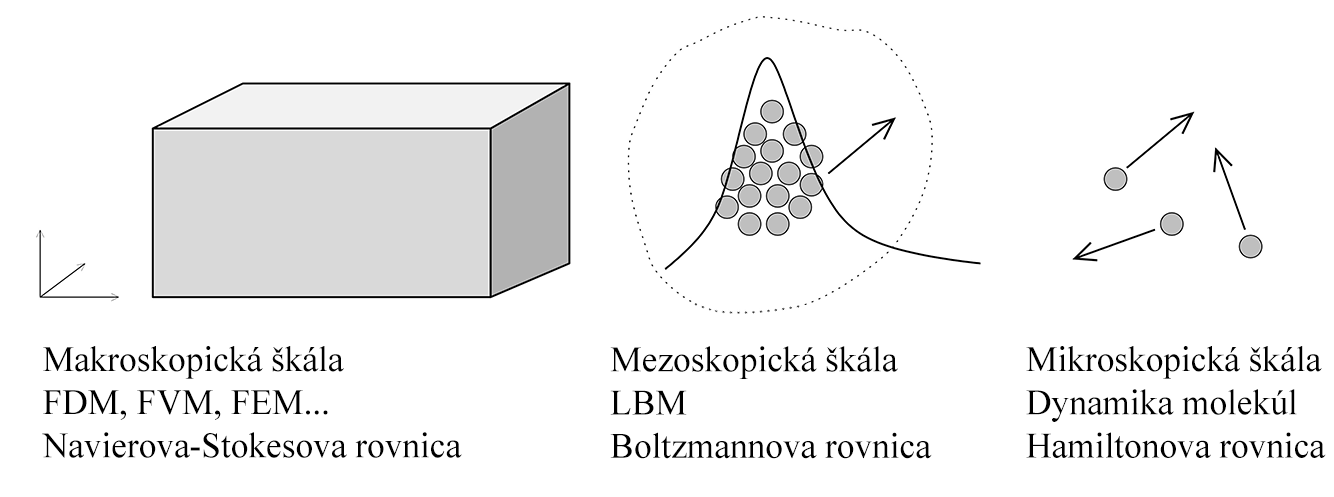
\includegraphics[width=1\textwidth,angle=0]{figures/different-scales.png}
	\caption{Techniky simulácie v rôznych škálach \citep{Mele2013}.}
\end{figure}

%The particles jump from one lattice node to the next, according to their (discrete) velocity. This is the propagation phase
Častice skočia z jedného mriežkového uzla do nasledujúceho podľa svojej (diskrétnej) rýchlosti. Toto je propagačná fáza

%Then, the particles collide and get a new velocity. This is the collision phase
Potom sa častice zrazia a získajú novú rýchlosť. Toto je fáza kolízie

%Rules governing the collisions are designed such that the time-average motion satisfies mass and momentum conservation
Pravidlá upravujúce zrážky sú navrhnuté tak, aby priemerný čas vyhovoval zachovaniu hmotnosti a hybnosti

\begin{figure}[!ht]
	\centering
	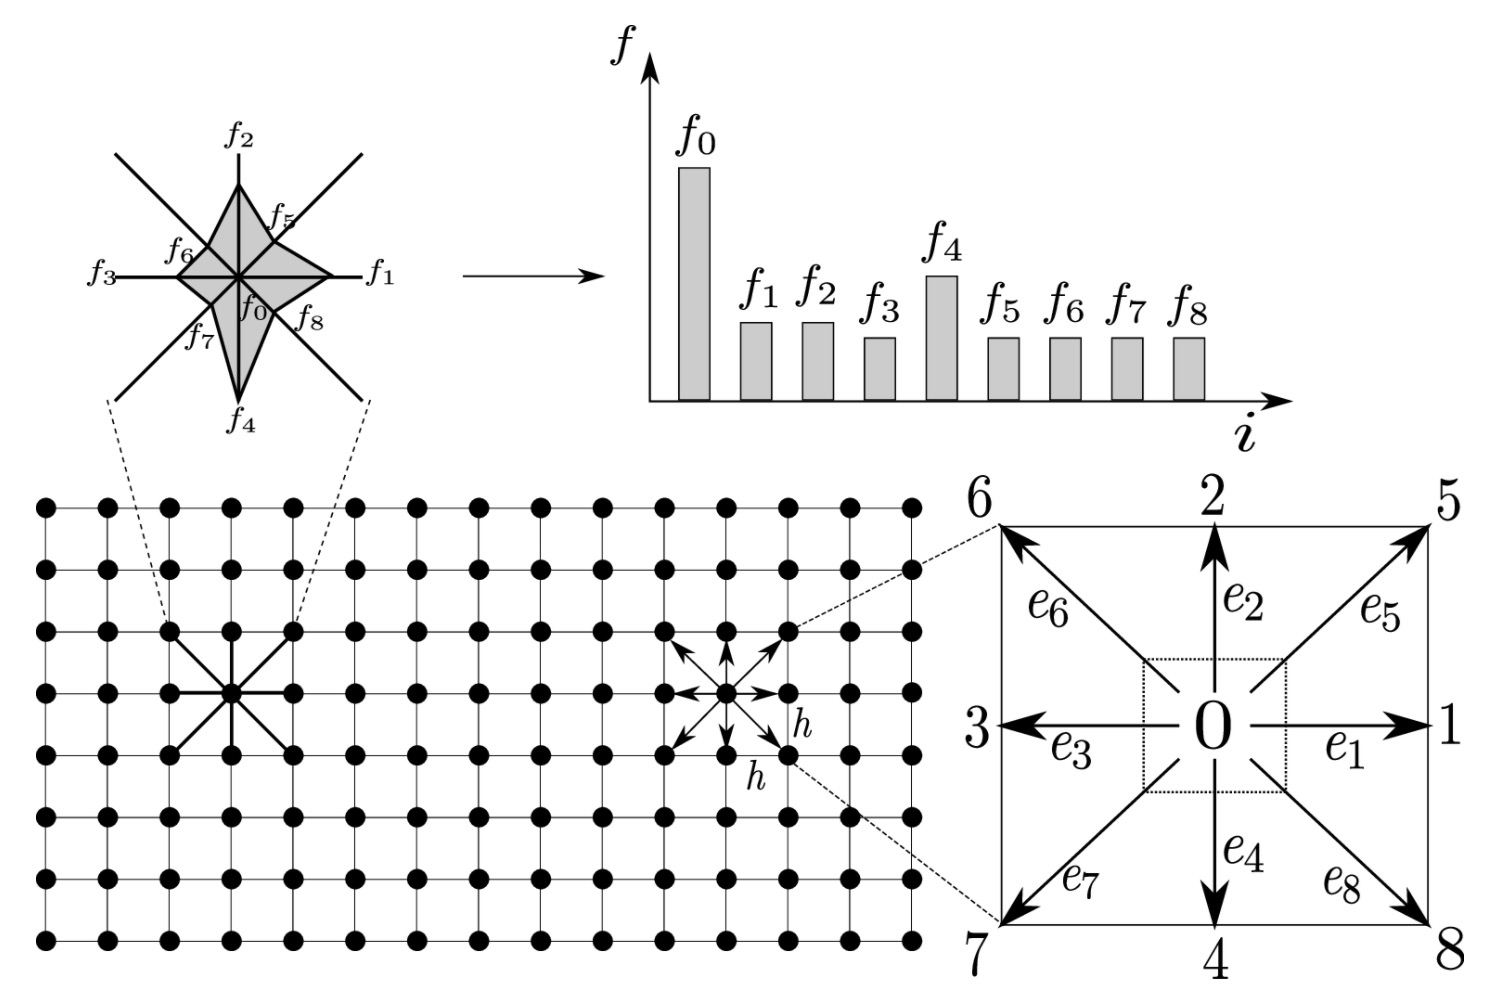
\includegraphics[width=.7\textwidth,angle=0]{figures/lbm-grid.jpg}
	\caption{Mriežková štruktúra LBM \citep{Soga2020}.}
\end{figure}

Pri LBM sa (ako aj pri iných numerických metódach) môže objaviť numerická nestabilita. Zatiaľ pre túto metódu nie sú presne dané podmienky stability, ale z doterajších praktických výpočtov vzišlo niekoľko podmienok, pri ktorých držaní sa je možné dosiahnuť akceptovateľnú stabilitu:

\begin{enumerate}
	\item{Kinetická viskozita by mala byť kladná.}
	\item{Výsledná makroskopická rýchlosť prúdenia}
\end{enumerate}


\subsection{Modelovanie turbulencie}

LES (Large Eddy Simulation) je matematický model turbulencie pôvodne navrhnutý Josephom Smagorinskym


$K-\epsilon$ je matematický model turbulencie

\subsection{DNS}

Direct Numerical Simulation

\section{Programy pre CFD simulácie}

\subsection{Matlab}
Matlab obsahuje niekoľko toolboxov pre CFD analýzu. 

\subsection{Ansys Fluid}

Ansys Fluid

\subsection{SimScale}

Platforma SimScale ponúka v rámci čiastkových produktov mnohé funkcionality ako ostatné simulačné programy, no táto firma stavila na využitie cloudových technológií. Práca s programom prebieha cez webové rozhranie, kde užívateľ nastavuje a spúšťa simulácie a taktiež sa priamo vo webovom prehliadači zobrazuje 2D alebo 3D vizualizácia simulovaného modelu. Výpočty prebiehajú na serveroch prevádzkovaných alebo prenajímaných firmou SimScale, ktoré využívajú možnosti masívnej paralelizácie grafických kariet


\begin{figure}[!ht]
	\centering
	\subfloat[Simulácia toku vetra okolo modelu niekoľkých výškových budov so zložitou geometriou.]{{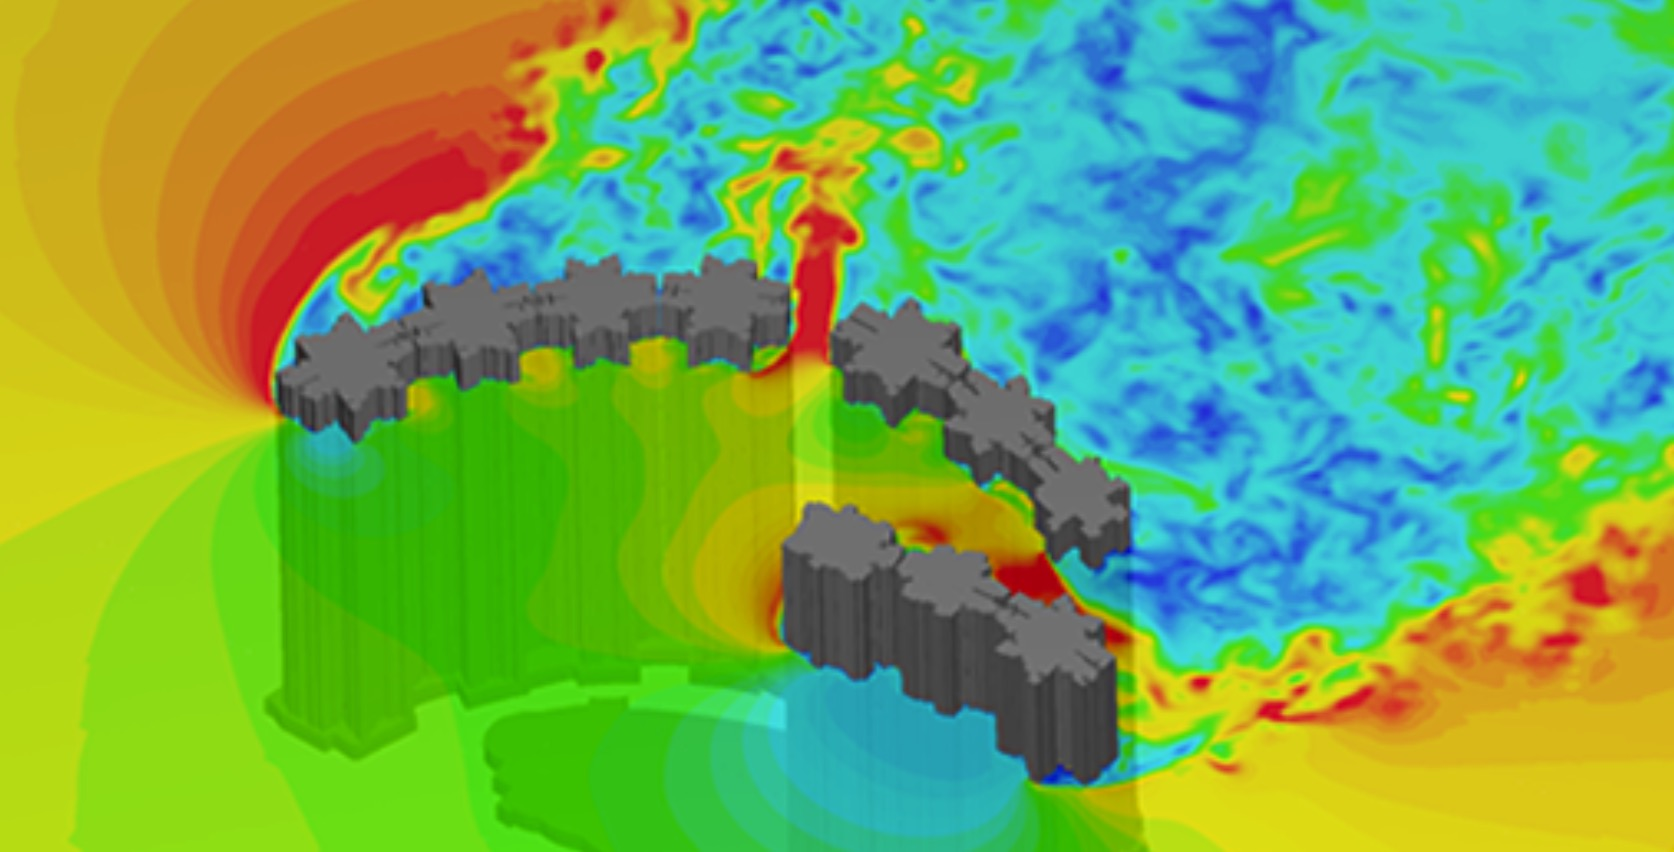
\includegraphics[width=7.1cm]{figures/simscale-cfd.jpg} }}%
	\qquad
	\subfloat[CFD simulácia viacfázovej tekutiny.]{{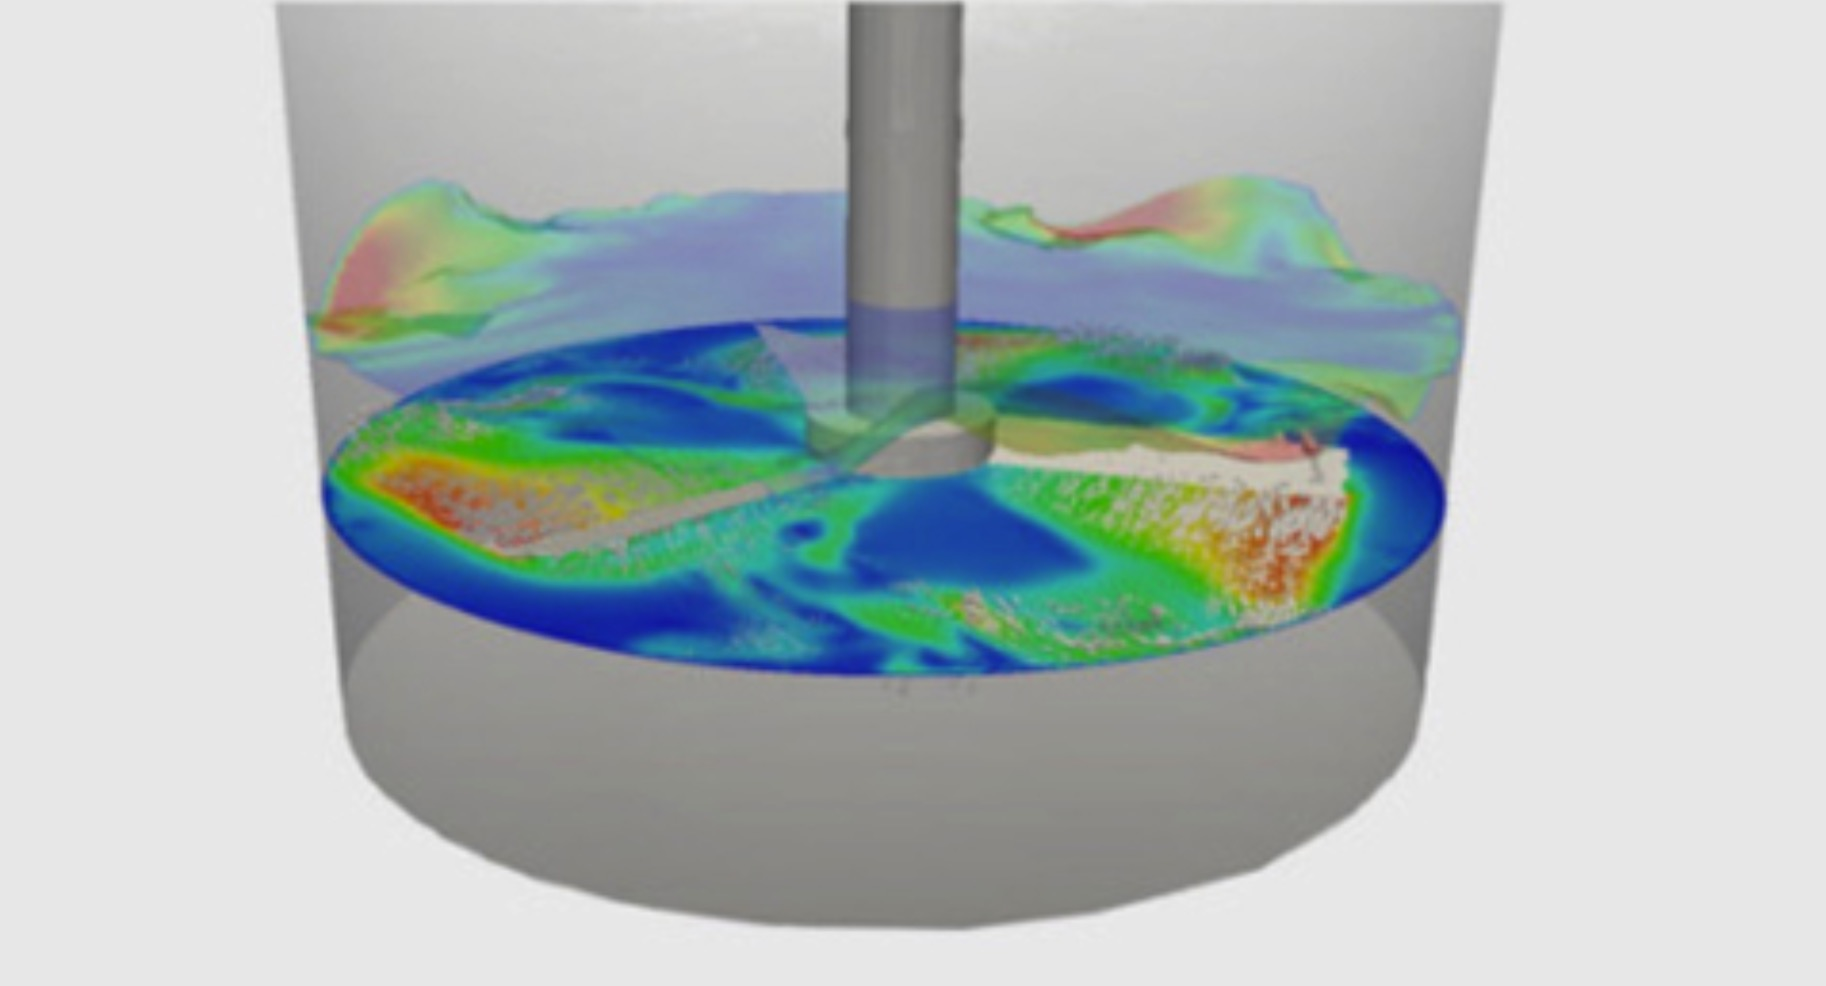
\includegraphics[width=6.7cm]{figures/simscale-multiphase.jpg} }}
	\caption{Vizualizácie CFD simulácií v prostredí SimScale.}
\end{figure}

\subsection{OpenFOAM}

%is a toolbox for solving complex Computational Fluid Dynamics problems. It contains a wide range of physical models (including turbulence, wall treatment, thermodynamics, and mass transport), numerical methods and tools for pre- and post-processing.

OpenFOAM je súbor nástrojov s voľne prístupným zdrojovým kódom na riešenie zložitých problémov s výpočtovou dynamikou tekutín. Obsahuje širokú škálu fyzikálnych modelov (vrátane turbulencie, úprav stien hraničných podmienok - geometrie, termodynamiky a hromadnej dopravy), numerických metód a nástrojov na predbežné a následné spracovanie.

\subsection{OpenLB}

OpenLB je balík C++ modulov pre implementáciu lattice Boltzmann simulácií určený predovšetkým ako programová podpora pre výskumníkov a technikov, ktorí simulujú toky tekutín pomocou LBM. Podporuje komplexné dátové štruktúry, pomocou ktorých je možné simulovať zložité geometrie. Diskretizovať geometrie (meshing alebo voxelizácia) z dopredu pripravených 3D modelov a nastaviť okrajové podmienky je možné automaticky - automatickým predspracovaním (aj komplexného) 3D modelu. Paralelizácia v implementovaných algoritmoch je riešená využitím knižnice OpenMP, z čoho môžu benefitovať výkonné multiprocesorové viacjadrové počítače (v architektúrach využívajúcich zdieľanú pamäť). Pri distribuovaných počítačových systémoch, na ktorých by sme chceli simulovať modely na báze LBM pomocou OpenLB majú paralelné algoritmy v tomto balíku implementované rozhranie na posielanie a prijímanie správ medzi jednotlivými procesmi (MPI - Message-Passing Interface

\section{Záver}

Simulácie sú v súčasnosti už neoddeliteľnou súčasťou počítačom podporovaného inžinierstva ako aj vedeckého skúmania fyzikálnych javov. Výsledkom simulácie je približné, no dostatočne presné riešenie modelovanej úlohy. Modelovanie na základe matematických metód prešlo dekádami vývoja a vylepšovanie metód pokračuje naďalej.  

%
%%
\Urlmuskip=0mu plus 1mu\relax
\bibliographystyle{spbasic}
\bibliography{refs/control,refs/mathematics,refs/modeling,refs/cfd,refs/lbm,refs/gpu,refs/interaction,refs/interfaces,refs/hci,refs/design,refs/ml,refs/visualization,refs/programming,refs/simulation,refs/ar,refs/vr,refs/online}

%

\end{document}
%%